\newpage\null\par
\section{实验三\hspace{1em}土壤环境质量现状调查}
\subsection{教学目的与要求}
\noindent\textbf{教学目的:}通过某校区实验楼建设项目为实例来进行土壤环境质量现状调查方案设计。
\newline\textbf{教学要求:} 
\begin{enumerate}
    \item 熟悉土壤环境质量监测布点及采样分析,能够根据影响识别结果与评价工作等,确定影响预测的范围、内容和方法。
    \item 根据最新版技术导则《环境影响评价技术导则——土壤环境(试行)》(HJ 964-2018)中的要求制定某校区实验楼建设项目的土壤环境质量现状监测方案(包含范围、布点(需要有实际现场布点图)、因子、方法、时期、次数等)。
\end{enumerate}


\subsection{实验报告背景}
\begin{enumerate}
    \item \textbf{建设项目类别:}\uppercase\expandafter{\romannumeral 2} 类 \\
    查阅《环境影响评价技术导则——土壤环境(试行)》(HJ 964-2018)附录A:对校区实验楼建设项目进行土壤环境影响评价时,发现并未找到与之相对应的行业类别区划,因此初步将其归类为其他行业,即 \uppercase\expandafter{\romannumeral 4} 类项目类别。然而,在进一步考虑时发现,校区实验楼一般包含化学试剂的处理和使用,这可能对土壤环境产生一定的影响。基于对土壤环境影响源、影响途径和影响因子的综合识别结果,我认为将该项目类别调整为 \uppercase\expandafter{\romannumeral 2} 类更为合理和符合逻辑。这样的调整考虑到了实验楼中存在的潜在化学物质对土壤环境的潜在影响,使评价结果更加全面准确。通过将项目类别归类为 \uppercase\expandafter{\romannumeral 2} 类,能够更好地识别和评估潜在的土壤环境风险,以便采取相应的环境保护措施和监测策略。

    \item \textbf{建设项目土壤环境影响类型:}污染影响型
    \begin{itemize}
        \item 建设期:在新建校区实验楼的建设期间,以下几种土壤环境影响类型可能发生:
        \begin{itemize}
            \item 大气沉降:建设期间可能会有空气中的颗粒物沉降到土壤中。
            \item 地面漫流:建设期间可能会有水流经过施工现场,携带土壤中的颗粒物等物质。
            \item 垂直入渗:施工期间可能使用水泥、混凝土等材料,其中的化学物质可能会渗入土壤中。
        \end{itemize}
        \item 运营期:运营期间通常不会有土壤环境影响,因为实验楼已经建成并投入使用。
        \item 服务期满后:在实验楼的服务期满后,通常也不会有土壤环境影响,因为实验楼已经停止使用。
    \end{itemize}
    \begin{table}[H]
        \centering
        \caption{建设项目土壤环境影响类型与影响途径表\cite{HJ964-2018}}
        \resizebox{\textwidth}{!}{
        \begin{tabular}{|c|c|c|c|c|c|c|c|c|}
        \hline
        \multirow{2}*{不同时段} & \multicolumn{4}{c|}{污染影响型}    & \multicolumn{4}{c|}{生态影响型} \\
        \cline{2-9}          & 大气沉降 & 地面漫流 & 垂直入渗 & 其他 & 盐化 & 碱化 & 酸化 & 其他 \\
        \hline
        建设期 & √ &  √ & √  &     &   &    &    &  \\
        \hline
        运营期 &   & &   &   &    &    &     &  \\
        \hline
        服务期满后 &   &    &   &    &    &    &    &  \\
        \hline
        \multicolumn{9}{|l|}{注:在可能产生的土壤环境影响类型处打“√”,列表未涵盖的可自行设计。} \\
        \hline
        \end{tabular}}
        \label{tab:Soil environmental impact types and impact pathways of construction projects}
    \end{table}

    \item 《土地利用现状分类》(GB/T 21010-2017)\textbf{建设项目土地利用现状分类和编码}:二级类,0803 教育用地。
    \item \textbf{建设项目占地规模:}小型($\leqslant 5$ hm$^2$)
    \item \textbf{建设项目所在地周边的土壤环境敏感程度:}敏感 \\
    校区实验楼位于学校的周边,因此建设项目需要特别关注学校土壤环境的敏感目标。
    \begin{table}[H]
        \centering
        \caption{污染影响型敏感程度分级表\cite{HJ964-2018}}
        \begin{tabular}{|c|l|}
            \hline
            敏感程度  & \multicolumn{1}{c|}{判别依据} \\
            \hline
            敏感    & \makecell[l]{建设项目周边存在耕地、园地、牧草地、饮用水水源地或居民区、\\学校、医院、疗养院、养老等土壤环境敏感目标的} \\
            \hline
            较敏感   & 建设项目周边存在其他土壤环境敏感目标的 \\
            \hline
            不敏感   & 其他情况 \\
            \hline
        \end{tabular}
        \label{tab:Contamination-affected sensitivity scale}
    \end{table}
    
    \item \textbf{建设项目评价工作等级:}二级
    \begin{table}[H]
        \centering
        \caption{污染影响型评价工作等级划分表\cite{HJ964-2018}}
        \resizebox{\textwidth}{!}{
        \begin{tabular}{|c|c|c|c|c|c|c|c|c|c|}
            \hline
            评价工作等级 & \multicolumn{3}{c|}{\uppercase\expandafter{\romannumeral 1}类} & \multicolumn{3}{c|}{\uppercase\expandafter{\romannumeral 2}类} & \multicolumn{3}{c|}{\uppercase\expandafter{\romannumeral 3}类} \\
            \hline
            \diagbox{敏感程度}{占地规模}  & 大 & 中 & 小 & 大 & 中 & 小 & 大 & 中 & 小 \\
            \hline
            敏感 & 一级 & 一级 & 一级 & 二级 & 二级 & \textcolor{orange}{二级} & 三级 & 三级 & 三级 \\
            \hline
            较敏感 & 一级 & 一级 & 二级 & 二级 & 二级 & 三级 & 三级 & 三级 & - \\
            \hline
            不敏感 & 一级 & 二级 & 二级 & 二级 & 三级 & 三级 & 三级 & - & - \\
            \hline
            \multicolumn{10}{|l|}{注:“-”表示可不开展土壤环境影响评价工作。} \\
            \hline
        \end{tabular}}
        \label{tab:Pollution impact assessment work classification table}
    \end{table}
\end{enumerate}


\subsection{报告主体内容}
\subsubsection{监测范围}

\paragraph{$\bullet $ 建设项目现状调查范围:}占地范围内:全部;占地范围外:0.2 km 范围内
\begin{table}[H]
    \centering
    \caption{现状调查范围\cite{HJ964-2018}}
    \begin{tabular}{|c|c|c|c|}
        \hline
        \multirow{2}*{评价工作等级} & \multirow{2}*{影响类型} & \multicolumn{2}{c|}{调查范围$\mathrm{^a}$} \\
        \cline{3-4}          &       & 占地$\mathrm{^b}$范围内 & 占地范围外 \\
        \hline
        \multirow{2}*{一级} & 生态影响型 & \multirow{6}*{\textcolor{orange}{全部}} & 5 km范围内 \\
        \cline{2-2}\cline{4-4}          & 污染影响型 &       & 1 km范围内 \\
        \cline{1-2}\cline{4-4}    \multirow{2}*{二级} & 生态影响型 &       & 2 km范围内 \\
        \cline{2-2}\cline{4-4}          & 污染影响型 &       &  \textcolor{orange}{0.2 km范围内} \\
        \cline{1-2}\cline{4-4}    \multirow{2}*{三级} & 生态影响型 &       & 1 km范围内 \\
        \cline{2-2}\cline{4-4}          & 污染影响型 &       & 0.05 km范围内 \\
        \hline
        \multicolumn{4}{|l|}{\small\makecell[l]{$\mathrm{^a}$涉及大气沉降途径影响的,可根据主导风向下风向的最大落地浓度点适当调整。\\$\mathrm{^b}$矿山类项目指开采区与各场地的占地;改、扩建类的指现有工程与拟建工程的占地。}} \\
        \hline
    \end{tabular}
    \label{tab:Scope of the current situation survey}
\end{table}
\normalsize

\paragraph{$\bullet $ 建设项目现状调查范围调整:}占地范围外:0.4 km 范围内 \par
校园实验楼通常提供各种化学品,以支持学生和教师在化学实验室进行实验和研究。这些化学品包括酸、碱、溶液、试剂、溶剂和实验用玻璃器皿等常见物品,旨在教学过程中帮助学生学习和实践化学实验技能。根据《环境影响评价技术导则——土壤环境(试行)》(HJ 964-2018)的规定,危险品、化学品或石油等输送管线的调查评价范围应从工程边界两侧向外延伸0.2公里。因此,在建设项目现状调查范围之外,调整范围应涵盖0.4公里以内的区域。这样的调整将更符合相关规定和要求。


\subsubsection{监测布点}

\paragraph{$\bullet $ 布点原则}~{}\par

由表 \ref{tab:Soil environmental impact types and impact pathways of construction projects} 可知,建设项目土壤环境影响途径有大气沉降、地面漫流和垂直入渗,再查阅《环境影响评价技术导则——土壤环境(试行)》(HJ 964-2018)得到相关布点原则如下:
\begin{enumerate}
    \item 涉及入渗途径影响的,主要产污装置区应设置柱状样监测点,采样深度需至装置底部与土壤接触面以下,根据可能影响的深度适当调整。
    \item 涉及大气沉降影响的,应在占地范围外主导风向的上、下风向各设置1个表层样监测点,可在最大落地浓度点增设表层样监测点。
    \item 涉及地面漫流途径影响的,应结合地形地貌,在占地范围外的上、下游各设置1个表层样监测点。
    \item 线性工程应重点在站场位置(如输油站、泵站、阀室、加油站及维修场所等)设置监测点,涉及危险品、化学品或石油等输送管线的应根据评价范围内土壤环境敏感目标或厂区内的平面布局情况确定监测点布设位置。
    \item 建设项目现状监测点设置应兼顾土壤环境影响跟踪监测计划。
\end{enumerate}


\paragraph{$\bullet $ 布点数量}~{}\par

从下表 \ref{tab:The type and number of current monitoring sites} 可知,二级污染影响型的现状监测布点类型与数量:
\begin{itemize}
    \item 占地范围内:3个柱状样点,1个表层样点
    \item 占地范围外:2个表层样点
\end{itemize}
\begin{table}[H]
    \centering
    \caption{现状监测布点类型与数量\cite{HJ964-2018}}
    \begin{tabular}{|c|c|c|c|}
        \hline
        \multicolumn{2}{|c|}{评价工作等级} & 占地范围内 & 占地范围外 \\
        \hline
        \multirow{2}*{一级} & 生态影响型 & 5个表层样点$\mathrm{^a}$ & 6个表层样点 \\
        \cline{2-4}          & 污染影响型 & 5个柱状样点$\mathrm{^b}$,2个表层样点 & 4个表层样点 \\
        \hline
        \multirow{2}*{二级} & 生态影响型 & 3个表层样点 & 4个表层样点 \\
        \cline{2-4}          & 污染影响型 & 3个柱状样点,1个表层样点 & 2个表层样点 \\
        \hline
        \multirow{2}*{三级} & 生态影响型 & 1个表层样点 & 2个表层样点 \\
        \cline{2-4}          & 污染影响型 & 3个表层样点 & - \\
        \hline
        \multicolumn{4}{|l|}{{\small 注:“-”表示无现状监测布点类型与数量的要求。}} \\
        \hline
        \multicolumn{4}{|l|}{\small\makecell[l]{$\mathrm{^a}$表层样应在 $0\sim 0.2$ m 取样。\\ $\mathrm{^b}$柱状样通常在 $0\sim 0.5$ m、$0.5\sim 1.5$ m、$1.5\sim 3$ m分别取样,3 m 以下每 3 m 取1个样,\\\phantom{$\mathrm{^b}$}可根据基础埋深、土体构型适当调整。}} \\
        \hline
    \end{tabular}
    \label{tab:The type and number of current monitoring sites}
\end{table}
\normalsize


\paragraph{$\bullet $ 布点方法}~{}\par
现状监测取样方法布点方法主要按照以下标准执行:\newline
$\bullet $ 《土壤环境监测技术规范》(HJ/T 166-2004)\newline
$\bullet $ 《建设用地土壤污染状况调查技术导则》(HJ 25.1-2019)\newline
$\bullet $ 《建设用地土壤污染风险管控和修复监测技术导则》(HJ 25.2-2019)

\begin{table}[H]
    \caption{几种常见的布点方法及适用条件\cite{HJ25.1-2019}}
    \centering
    \resizebox{\textwidth}{!}{
    \begin{tabular}{|c|l|}
        \hline
        布点方法 & \multicolumn{1}{|c|}{适用条件}  \\
        \hline
        系统随机布点法 & 适用于污染分布均匀的地块。\\
        \hline
        专业判断布点法 & 适用于潜在污染明确的地块。\\
        \hline
        分区布点法 & 适用于污染分布不均匀,并获得污染分布情况的地块。\\
        \hline
        系统布点法 & 适用于各类地块情况,特别是污染分布不明确或污染分布范围大的情况。\\
        \hline
    \end{tabular}}
    \label{tab:Several common distribution methods and applicable conditions}
\end{table}

\begin{figure}[H]
    \centering
    \begin{subfigure}[h]{0.3\textwidth}
        \centering
        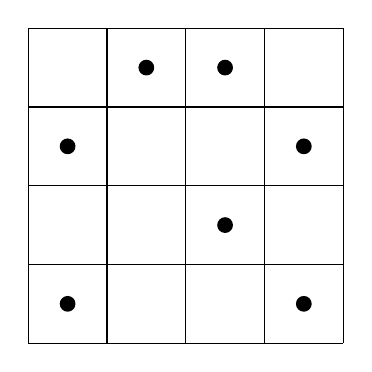
\begin{tikzpicture}
            \draw[step=1cm] (0,0) grid (4,4);
            \foreach \x/\y in {0/0,1/3,2/3,3/2,2/1,3/0,0/2} {
                \fill[black] ({\x+0.5},{\y+0.5}) circle (0.1cm);
            }
        \end{tikzpicture}
        \caption{系统随机布点法}
    \end{subfigure}
    \hfill
    \begin{subfigure}[h]{0.3\textwidth}
        \centering
        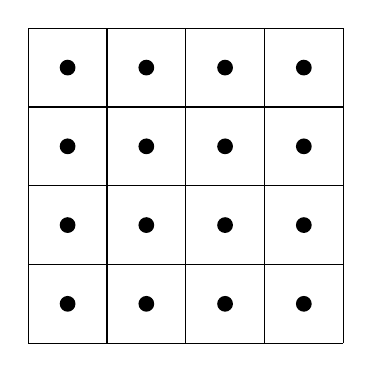
\begin{tikzpicture}
            \draw[step=1cm] (0,0) grid (4,4);
            \foreach \x in {0,1,2,3} {
                \foreach \y in {0,1,2,3} {
                    \fill[black] ({\x+0.5},{\y+0.5}) circle (0.1cm);
                }
            }
        \end{tikzpicture}
        \caption{系统布点法}
    \end{subfigure}
    \hfill
    \begin{subfigure}[h]{0.3\textwidth}
        \centering
        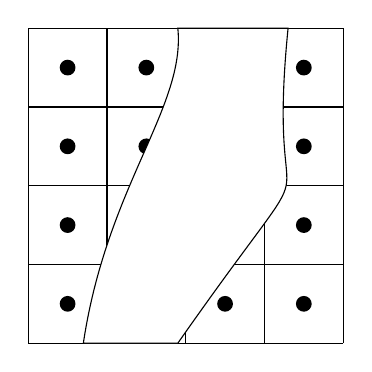
\begin{tikzpicture}
            \draw[step=1cm] (0,0) grid (4,4);
            \foreach \x in {0,1,2,3} {
                \foreach \y in {0,1,2,3} {
                    \fill[black] ({\x+0.5},{\y+0.5}) circle (0.1cm);
                }
            }
            \draw[smooth, fill=white] (0.7,0) .. controls (1,2) and (2,3) .. (1.9,4) -- ++(1.4,0) .. controls (3,1) and (4,3) .. (1.9,0) -- cycle;
        \end{tikzpicture}
        \caption{分区布点法}
    \end{subfigure}
    \caption{监测点位布设方法示意图\cite{HJ25.2-2019}}
    \label{fig:Soil monitoring point layout method (commonly used)}
\end{figure}

如图 \ref{fig:Soil monitoring point layout method (commonly used)} 和表 \ref{tab:Several common distribution methods and applicable conditions} 所示,常用的土壤监测点位布设方法有多种,分别是系统随机布点法、专业判断布点法、系统布点法、分区布点法。考虑到校区实验楼建设项目地块土壤污染特征不明确,则采用系统布点法进行监测点位布设。系统布点法是将监测区域分成面积相等的若干工作单元,每个工作单元内布设一个监测点位。

查阅《建设用地土壤污染风险管控和修复监测技术导则》(HJ 25.2-2019),单个工作单元的面积可根据实际情况确定,原则上不应超过 1600 m$^2$。对于面积较小的地块,应不少于5个工作单元。

\paragraph{$\bullet $ 监测布点图}~{}\par

以成都理工大学宜宾校区实验楼建设为项目例子,查阅中国气象局,四川宜宾的常年风向是东南风和西南风。考虑风向布点如下:
\begin{figure}[H]
    \centering
    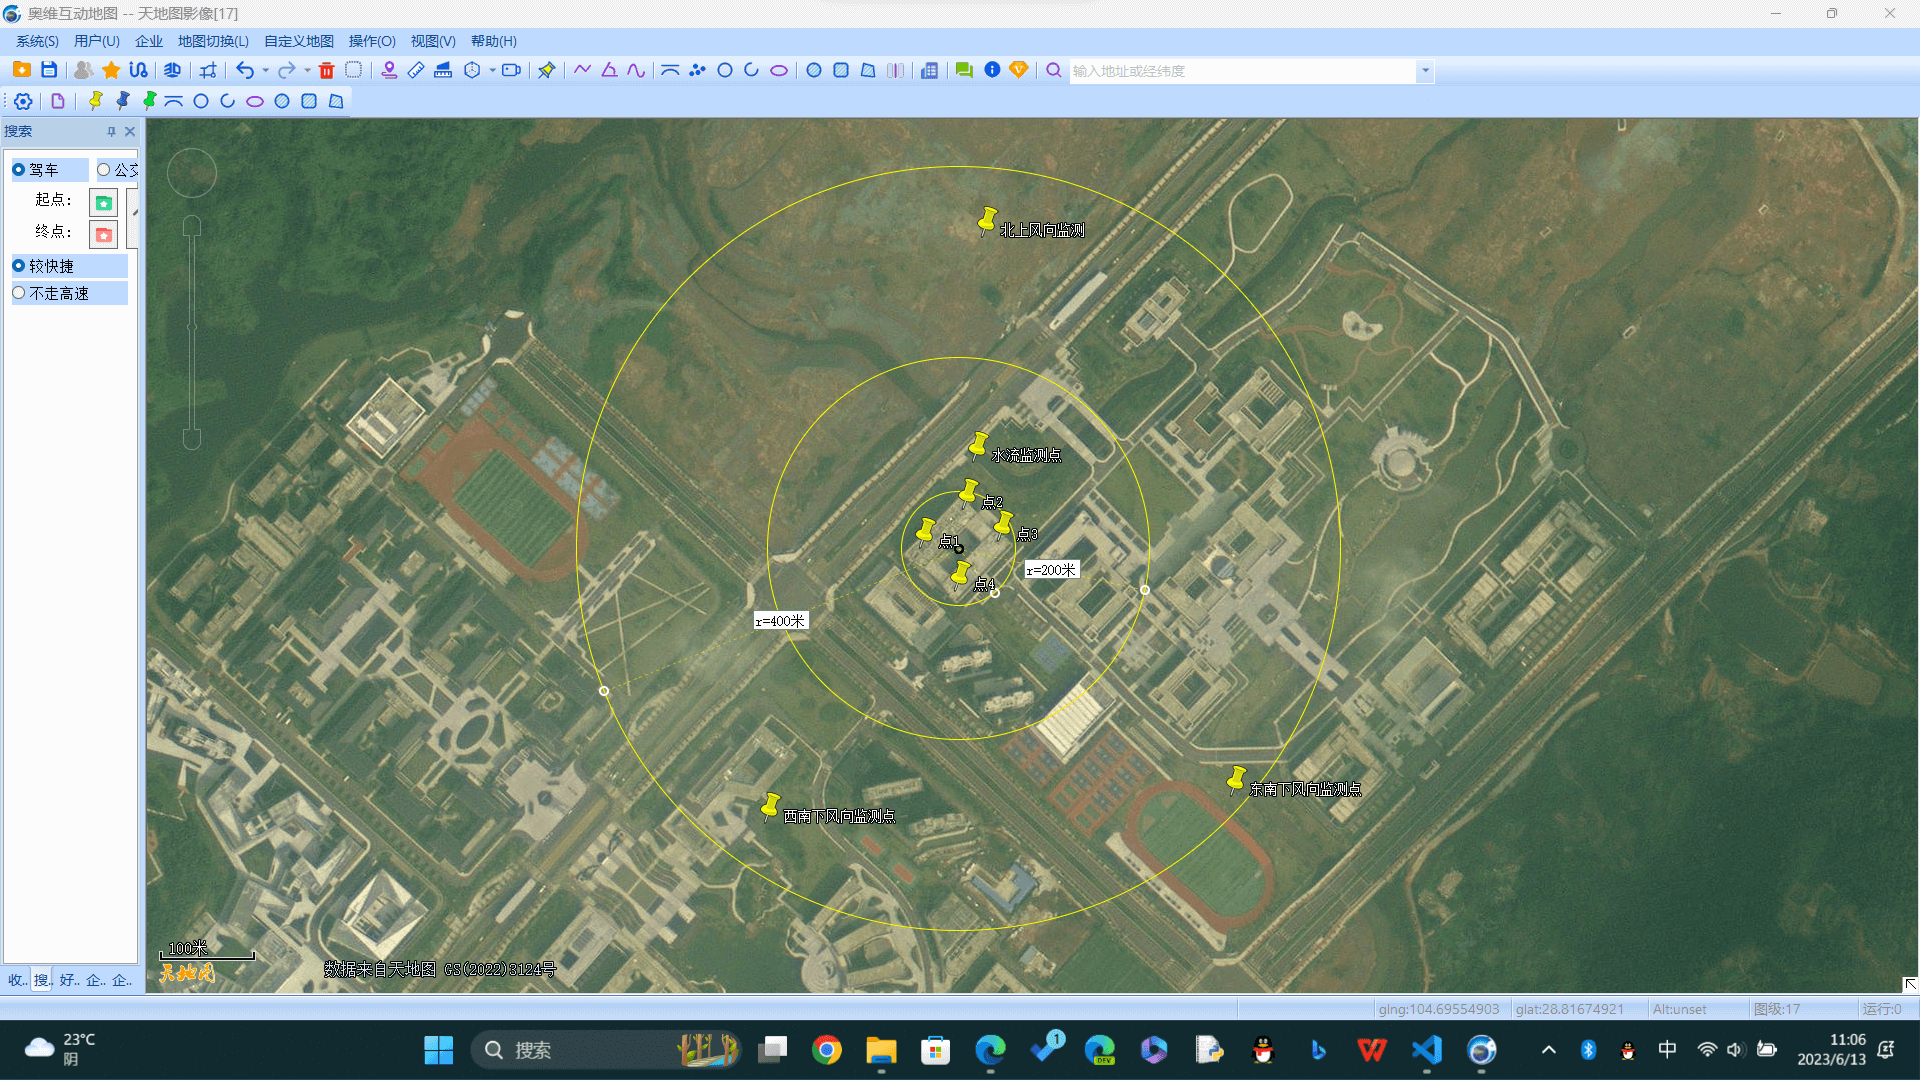
\includegraphics[width=\textwidth]{figures/Soil monitoring dot map.png}
    \caption{土壤监测布点图}
    \label{fig:Soil monitoring dot map}
\end{figure}

如图 \ref{fig:Soil monitoring dot map} 所示,一共设置了8个监测点:

在项目建设期间,由于可能产生大气沉降污染,建议在项目占地范围外,根据主导风向的上风向和下风向各设置至少一个表层样本监测点。根据中国气象局的数据显示,四川宜宾地区的常年风向主要为东南风和西南风。因此,在上风向方向应设立一个监测点,而在下风向方向则建议设置两个监测点。这样的设置可以更全面地监测大气沉降污染情况,确保项目对环境的影响能够得到及时有效的评估和控制。
\begin{itemize}
    \item 北上风向监测 $(g104^{\circ}41'22.52'',28^{\circ}49'14.55'')$:选择这个监测点是为了监测来自北方的风向,这样可以了解北方是否存在潜在的污染源,并对风向的变化进行监测。
    \item 西南下风向监测点 $(g104^{\circ}41'14.11'',28^{\circ}48'54.69'')$:选择这个监测点是为了监测来自西南方向的风向。西南下风向是项目占地区域内可能受到污染物影响的方向,监测此处可以提供关于污染物传播的重要信息。
    \item 东南下风向监测点 $(g104^{\circ}41'32.16'',28^{\circ}48'55.64'')$:选择这个监测点是为了监测来自东南方向的风向。东南下风向也是项目占地区域内可能受到污染物影响的方向,监测此处可以提供关于污染物传播的重要信息。
\end{itemize}

针对可能对地面漫流途径产生影响的情况,建议根据地形地貌,在项目占地范围外的上游和下游各设置一个表层样本监测点。然而,鉴于范围内的河流面积相对较小,所以在水流的中点只设置了一个监测点。
这样的监测点布置策略将有助于全面评估地面漫流途径可能带来的影响,并结合地形地貌因素进行合理的监测点位置选择。通过在上游和下游各设置一个监测点,可以有效监测沿水流方向的潜在影响。虽然范围内的河流面积较小,但在水流中点设置监测点可以提供对整体情况的综合评估。
\begin{itemize}
    \item 水流监测点 $(g104^{\circ}41'22.17'',28^{\circ}49'6.93'')$:选择这个监测点是为了监测水流的方向和流速。水流的监测对于了解水体中的污染物传播和扩散非常重要,可以帮助评估污染物对土壤的影响范围。
\end{itemize}

% 系统布点法通常基于以下原则:首先,在区域内选择均匀分布的点,以覆盖整个区域,并保证结果的代表性。其次,考虑到可能存在的污染源或潜在的影响区域,选择在可能受到污染物影响的位置进行监测。点1到点4的选择则是根据这些原则确定的,以确保有效监测土壤中的污染情况。
系统布点法通常基于以下原则进行设计和选择监测点。首先,要确保在区域内选择均匀分布的监测点,以覆盖整个区域并保证结果的代表性。其次,需要考虑潜在的污染源或可能受到污染物影响的区域,以选择适当的监测位置。
在本案例中,点1到点4的选择是基于这些原则确定的,旨在有效监测土壤中的污染情况。通过均匀分布这些监测点,可以全面覆盖整个区域并确保监测结果的可靠性。同时,这些点的位置选择还考虑了可能存在的污染源或潜在的影响区域,以确保对可能受到污染物影响的地区进行监测。
使用系统布点法能够帮助您有效评估土壤污染情况,并为制定相应的环境保护和修复策略提供准确的数据支持。
\begin{itemize}
    \item 点1: $(g104^{\circ}41'20.11'',28^{\circ}49'4.01'')$
    \item 点2: $(g104^{\circ}41'21.78'',28^{\circ}49'5.32'')$
    \item 点3: $(g104^{\circ}41'23.13'',28^{\circ}49'4.24'')$
    \item 点4: $(g104^{\circ}41'21.49'',28^{\circ}49'2.56'')$
\end{itemize}



\subsubsection{监测因子}
\paragraph{$\bullet $ 基本因子}~{}\par
因为土地利用为建设用地,所以遵循《土壤环境质量——建设用地土壤污染风险管控标准(试行)》(GB 36600-2018),然后校园实验楼项目又可以细分为第一类用地:公共管理与公共服务用地中的中小学用地(A33)。根据其中的建设用地土壤污染风险筛选值和管制值(基本项目)表格可以选定三个常规重金属为污染物项目作为土壤环境现状监测基本因子:
\begin{table}[H]
    \centering
    \caption{土壤环境现状监测基本因子\cite{GB36600-2018}}
    \begin{tabular}{cccc}
    \multicolumn{4}{r}{单位:mg/kg} \\
    \toprule
    污染物项目 & CAS 编号 & 筛选值   & 管制值 \\
    \midrule
    铬(六价) & 18540-29-9 & 3.0   & 30 \\
    铜     & 7440-50-8 & 2000  & 8000 \\
    铅     & 7439-92-1 & 400   & 800 \\
    \bottomrule
    \end{tabular}
    \label{tab:Basic factors for monitoring the status of soil environment}
\end{table}

\paragraph{$\bullet $ 特征因子}~{}\par
如表 \ref{tab:Soil environmental impact types and impact pathways of construction projects} 所示,可以设置项目特征因子为大气沉降、地面漫流、垂直入渗的监测因子。



\subsubsection[监测方法]{监测方法\cite{HJ25.2-2019}}
\paragraph{$\bullet $ 表层土壤样品的采集}~{}\par
\begin{enumerate}
    \item 表层土壤样品的采集一般采用挖掘方式进行,一般采用锹、铲及竹片等简单工具,也可进行钻孔取样。
    \item 土壤采样的基本要求为尽量减少土壤扰动,保证土壤样品在采样过程不被二次污染。
\end{enumerate}

\paragraph{$\bullet $ 下层土壤样品的采集}~{}\par
\begin{enumerate}
    \item 下层土壤的采集以钻孔取样为主,也可采用槽探的方式进行采样。
    \item 钻孔取样可米用人上心螺旅钻、中空螺旋钻、套管钻等。据他断而管式采样器等。机械钻探包括实心螺旋钻、中空螺旋钻、套管钻等。
    \item 槽探一般靠人工或机械挖掘采样槽,然后用采样铲或采样刀进行采样。槽探的断面呈长条形,根据地块类型和采样数量设置一定的断面宽度。槽探取样可通过锤击敞口取土器取样和人工刻切块状土取样。
\end{enumerate}

\paragraph{$\bullet $ 下层土壤样品的采集}~{}\par
挥发性有机物污染、易分解有机物污染、恶臭污染土壤的采样,应采用无扰动式的采样方法和工具。钻孔取样可采样快速击入法、快速压入法及回转法,主要工具包括土壤原状取土器和回转取土器。槽探可采用人工刻切块状土取样。采样后立即将样品装入密封的容器,以减少暴露时间。

\paragraph{$\bullet $ 土壤混合样的采集}~{}\par
如需采集土壤混合样时,将等量各点采集的土壤样品充分混拌后四分法取得到土壤混合样。含易挥发、易分解和恶臭污染的样品必须进行单独采样,禁止对样品进行均质化处理,不得采集混合样。

\paragraph{$\bullet $ 土壤样品的保存与流转}~{}\par
\begin{enumerate}
    \item 挥发性有机物污染的土壤样品和恶臭污染土壤的样品应采用密封性的采样瓶封装,样品应充满容器整个空间;含易分解有机物的待测定样品,可采取适当的封闭措施(如甲醇或水液封等方式保存于采样瓶中)。样品应置于4℃以下的低温环境(如冰箱)中运输、保存,避免运输、保存过程中的挥发损失,送至实验室后应尽快分析测试。
    \item 挥发性有机物浓度较高的样品装瓶后应密封在塑料袋中,避免交叉污染,应通过运输空白样来控制运输和保存过程中交叉污染情况。
    \item 具体土壤样品的保存与流转应按照 HJ/T 166的要求进行。
\end{enumerate}

\paragraph{$\bullet $ 土壤样品分析}~{}\par
土壤样品关注污染物的分析测试应参照 GB 36600 和 HJ/T 166 中的指定方法。土壤的
常规理化特征土壤 pH、粒径分布、密度、孔隙度、有机质含量、渗透系数、阳离子交换量
等的分析测试应按照 GB 50021 执行。污染土壤的危险废物特征鉴别分析,应按照 GB 5085
和 HJ 298 中的指定方法。

\paragraph{$\bullet $ 监测因子分析方法}~{}\par
\begin{table}[H]
    \centering
    \caption{土壤污染物分析方法}
    \begin{tabular}{ccc}
    \toprule
    污染物项目  & 分析方法  & 标准编号 \\
    \midrule
    铬(六价)  & 火焰原子吸收分光光度法 & HJ 491-2019 \\
    铜      & 火焰原子吸收分光光度法 & HJ 491-2019 \\
    铅     & 火焰原子吸收分光光度法 & HJ 491-2019 \\
    \bottomrule
    \end{tabular}
    \label{tab:Methods for soil pollutant analysis}
\end{table}



\subsubsection{监测时期}

根据《土壤环境监测技术规范》(HJ/T 166-2004)要求,可以选定监测时期为污染物更为容易扩散的夏季。

\begin{table}[H]
    \centering
    \caption{土壤监测项目与监测频次\cite{HJ/T166-2004}}
    \begin{tabular}{|c|c|c|c|}
    \hline
    \multicolumn{2}{|c|}{项目类别} & 监测项目  & 监测频次 \\
    \hline
    \multirow{2}*{常规项目} & 基本项目  & pH、阳离子交换量 & \multirow{2}*{\makecell[l]{每3年一次\\农田在夏收或秋收后采样}} \\
    \cline{2-3}          & 重点项目  &  \makecell[l]{镉、铬、汞、砷、铅、铜、\\锌、镍、六六六、滴滴涕} &  \\
    \hline
    \multicolumn{2}{|c|}{特定项目(污染事故)} & 特征项目  & \makecell[l]{及时采样,根据污染物\\变化趋势决定监测频次} \\
    \hline
    \end{tabular}
    \label{tab:Soil monitoring projects and monitoring frequency}
\end{table}
  



\subsubsection{监测次数}
\begin{enumerate}
    \item 基本因子:该建设项目的评价工作等级为为二级,每3年至少1次的监测数据;
    %引用监测数据应满足7.4.2和7.4.3的相关要求,并说明数据有效性;
    \item 特征因子:应至少开展1次现状监测。
\end{enumerate}



\subsection{小结及建议}

制定某校区实验楼建设项目的土壤环境质量现状监测方案是确保项目建设与环境保护的重要环节。通过科学合理的监测方案,可以及时发现和评估土壤环境质量变化情况,采取相应的措施保护土壤资源和生态环境。

在上面的现状监测方案制定中,提出了确定监测范围、布点设计、监测因子、监测方法、监测时期和次数等关键步骤和考虑因素。这些措施将有助于评估实验楼建设对土壤环境的影响,及时采取相应的保护和修复措施。同时,强调了代表性和充分覆盖原则在布点设计中的重要性,以确保监测结果的可靠性和代表性。

最后,制定和执行土壤环境质量现状监测方案应与相关法律法规和标准保持一致,确保建设项目符合环境保护的要求,为校区实验楼建设提供科学依据和环境保障。

